%author         Claus 
%1st review     Søren
%2nd review     Troels
\chapter{Time Division Multiple Access}\label{TDMA}

\gls{tdma} is a channel access method used for sharing the same radio frequency between two or more devices.
This method was first used in practice in 1991 for use in the cellular telephone to increase the number of concurrent users on the telephone network, according to \citet{networkencyclopedia2013time}.

This method is a great starting point when designing the network of this paper.
In the following section further explanation of \gls{tdma} is given.

\section{How TDMA works}

\begin{SCfigure}
    \vspace{-10pt}
    \centering
    \footnotesize
    \resizebox{0.5\linewidth}{!}{%
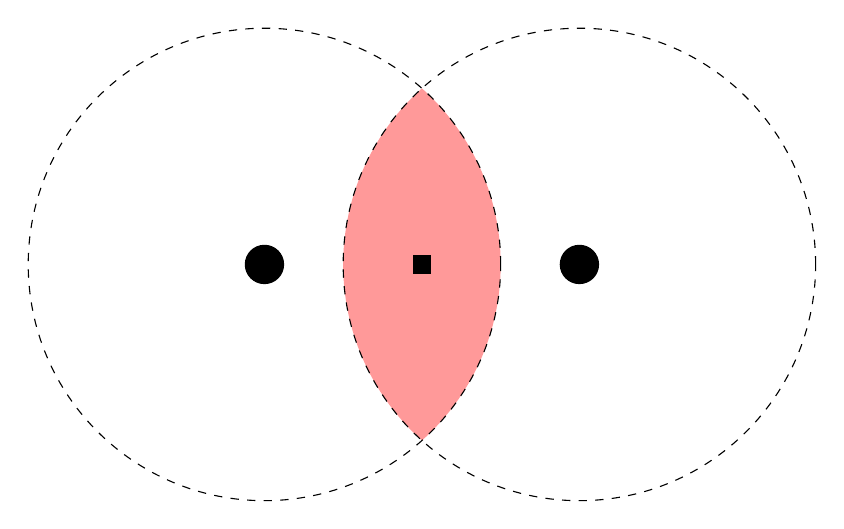
\begin{tikzpicture}
    \begin{scope}
        \clip (0,0) circle (3);
        \fill[red!40] (4,0) circle (3);
    \end{scope}

    \fill (0,0) circle (0.25);
    \draw[dashed] (0,0) circle (3);
    
    \fill (4,0) circle (0.25);
    \draw[dashed] (4,0) circle (3);
    
    \node[fill] at (2,0) {};
\end{tikzpicture}}
    \caption{The two devices (circles) transmitting on the same frequency making the receiver (square) unable to read either signal.}
    \label{fig:rangediagram}
    \vspace{-10pt}    
\end{SCfigure}

If multiple radio devices transmit on the same frequency at the same time while within the range of each other interference occurs, as can be seen on \myref{fig:rangediagram}. 
On the figure the device denoted by a square is within the range of both the devices denoted by circles. 
If they broadcast on the same frequency at the same time, what is called a collision occurs, then the square device will not be able to decode either of the signals \cite{networkencyclopedia2013time, networkencyclopedia2013advanced}.
When a collision occurs the transmission is jammed and should be avoided in all cases if possible.


\gls{tdma} addresses this problem by having the devices take turns transmitting their message in allocated time slots as seen on \myref{fig:tdmaoverview}.
The figure shows five devices which share the same frequency, and to do this, they get a time-slot each in the frame.
A frame is the complete cycle of these time-slots.

\tikzfigure{TDMAOverview.tex}{An example of a time slot allocation for five devices on a single frequency by using \gls{tdma}.}{tdmaoverview} %label: fig:tdmaoverview 

\noindent
Just like frames are divided into time slots; the following five parts are what the individual time slots consists of:

\begin{description}[labelindent=\parindent]
	\item[Guard time]\hfill\\ 
	A period where no important data is sent.
	This is here to make sure that devices not synchronised to the loop are less likely to corrupt the signal of other senders.

	\item[Sync]\hfill\\ 
	A possible extra delay before the signal depending on the distance to the receiver.

	\item[Control]\hfill\\
	One or more control values which determine the nature of the signal. 
	This could be message type, the length of the message, receiver, etc.

	\item[Data]\hfill\\
	The main data of the message.

	\item[\acrshort{crc} check]\hfill\\
	The \gls{crc} is an error-detecting code. 
	It is there to state whether the message received was corrupted, or not. 
\end{description}

\bigskip
\noindent
The aim of these divisions is to isolate each device, so that no jam occurs, and make sure that issues due to noise are minimised. 